\chapter{Development of Synthetic Smokers}
\label{ch:synthetic-smoker}

The iterative development of MIBot, as described in (Chapter~\ref{ch:mibot}), required that we extensively test it after every change in its prompt. To automate the testing of some aspects of the chatbot's behaviour, we started the development of ``synthetic smokers.''\footnote{It is worth mentioning that we also utilized human role-playing as smokers during our testing of MIBot.} A Synthetic Smoker, in the context of this research, is a prompted instance of an LLM tasked to simulate the behaviour, language, and psychological responses of a human smoker engaged in a counselling session.

This chapter details the conceptualization, iterative development, and validation of these synthetic agents.

\section{Objectives and Overview}
\label{sec:synthetic-smoker-goals}

The overarching goal of developing synthetic smokers is to create realistic and controllable stand-ins for human participants. This endeavour serves two primary objectives:

\begin{enumerate}
    \item \textbf{Testing Automated Systems:} Synthetic smokers provide a platform for the rapid iterative development and testing of automated counselling chatbots. By simulating interactions, developers may identify weaknesses, refine conversational strategies, and assess potential efficiency without the logistical overhead of recruiting human subjects for every iteration.
    \item \textbf{Training Human Clinicians:} In the role of standardized patients, synthetic smokers can be used to train novice clinicians. They offer a consistent experience and can be programmed to simulate specific challenging scenarios or diverse demographic profiles, which could help trainees receive varied practice opportunities.
\end{enumerate}

The development of a truly representative synthetic smoker poses a scientific challenge. It requires not only the generation of coherent dialogue but the accurate embodiment of specific human attributes ranging from demographics to complex psychological states like resistance to change. Crucially, the validation of these synthetic agents (i.e., proving that they behave realistically according to their installed attributes) is exceptionally difficult, as establishing the \textit{construct validity} of behavioural measurements remains a persistent challenge; that is, it is difficult to ensure that an instrument truly measures the specific psychological attribute it purports to assess \cite{Cronbach1955}.


\section{Defining the Ideal Synthetic Smoker}
\label{sec:synthetic-smoker-ideal}

In an ideal scenario, a synthetic smoker would be indistinguishable from a human participant within the constrained context of a smoking cessation counselling session. This requires the synthetic agent to possess a defined set of attributes and for those attributes to be reliably reflected in its interactions and behaviours.

We conceptualize a synthetic smoker based on a collection of attributes that define a human smoker. These attributes can be broadly categorized as:

\begin{itemize}
    \item \textbf{Demographic:} age, sex, education level, cultural background, etc.
    \item \textbf{Behavioural:} smoking history (e.g., Heaviness of Smoking Index (HSI)), previous quit attempts, verbosit, etc.
    \item \textbf{Psychological:} resistance to change, motivation levels (e.g., operationalized by pre-conversation readiness rulers), underlying values.
\end{itemize}

A successful system (or methodology) for creating synthetic smokers must produce agents that exhibit both high \emph{fidelity} and \emph{representativeness}.

\textbf{Fidelity} refers to the requirement that any attribute installed in the synthetic smoker must be demonstrably evidenced by its language and behaviour. For example, if a synthetic smoker is installed with high resistance, its dialogue should contain more sustain talk than change talk. The core challenge of this research is to develop methods to install these attributes and subsequently validate that this installation was successful.

\textbf{Representativeness} encompasses two key requirements. 

\begin{enumerate}
    \item First, the system must generate a diverse range of smokers whose attributes mirror the variability of the target real-world population. It must avoid the bias of over-representing a narrow or easily simulated archetype at the expense of mirroring the population's true statistical makeup. This may happen for a variety of reasons. For example, if the system is built on biased data, it may fail to generate a statistically accurate population.

    \item Second, the smokers created by the system should exhibit uniform fidelity, i.e., it should not have performance biases where specific profiles are simulated more accurately than others. A system might, for instance, be highly effective at simulating a 55-year-old, heavily dependent smoker with low motivation to quit, while failing to simulate a 22-year-old ``social smoker'' who is ambivalent about quitting. Representativeness requires that the quality of the simulation remains high across the entire spectrum of generated profiles.
\end{enumerate}



Let the collection of all relevant attributes define an $n$-dimensional \emph{attribute space}, $\mathcal{A}$. A specific smoker's profile, whether human or synthetic, is a vector $\textbf{A}$ within this space.
$$\textbf{A} = (a_1, a_2, \ldots, a_n) \in \mathcal{A}$$

The \emph{observable output space}, $\Gamma$, contains all possible outputs from a counselling session, such as conversation transcripts and survey responses. A specific session's output is an element $\gamma \in \Gamma$.
$$\gamma = \{\text{Transcript}, \text{Survey Responses}, \ldots\}$$

Human behaviour is not deterministic; a human $H$ with a given attribute vector $\textbf{A}_H$ will not produce the exact same output in every session. Instead, their behaviour is better modelled as a sample from a conditional probability distribution, $P_H(\gamma | \textbf{A}_H)$. Consequently, a synthetic smoker system, $S$, should not be a deterministic function but a model that approximates this human distribution, $P_S(\gamma | \textbf{A}_S)$. The goal is to ensure that $P_S(\gamma | \textbf{A}) \approx P_H(\gamma | \textbf{A})$.

To assess whether the system has achieved this goal, we must formalize the process of validation. For this, we define a \emph{measurement function}, $M$, that takes an output $\gamma$ and returns an estimated attribute vector $\hat{\textbf{A}}$.

$$M: \Gamma \rightarrow \mathcal{A}, \quad \text{where} \quad \hat{\textbf{A}} = M(\gamma)$$

For example, $M$ could be a set of classifiers and analytical tools that read a transcript and analyze post-conversation changes in behaviour to estimate the speaker's resistance, motivation, smoking history, etc., and produce  $\hat{\textbf{A}}$. It is worth mentioning that the measurement function $M$ is an imperfect proxy, as inferring latent constructs from observable behaviour is a persistent challenge in psychometric theory \cite{loevinger1957objective, borsboom2004concept}.

\subsection{Defining Fidelity}

Fidelity measures how accurately the observable outputs of a synthetic smoker reflect its assigned attributes. High fidelity is achieved when the attributes measured from the output, $\hat{\textbf{A}}_S = M(\gamma_S)$, are close to the input attributes, $\textbf{A}_S$. We quantify this correspondence using a distance metric, $d(\textbf{A}_S, \hat{\textbf{A}}_S)$, in the attribute space.

Given the stochastic nature of the generative system, a single instance is insufficient for evaluation. We therefore define the fidelity for a profile $\textbf{A}_S$ as the \emph{expected distance} between the input and measured attributes over the distribution of all possible outputs.
$$\mathcal{F}(\textbf{A}_S) = \mathbb{E}_{\gamma_S \sim P_S(\gamma | \textbf{A}_S)}[d(\textbf{A}_S, M(\gamma_S))]$$
A lower value of $\mathcal{F}(\textbf{A}_S)$ indicates higher fidelity. The objective of the system, then, is to minimize this value across all possible profiles.

In practice, one may not need $M$ to calculate the fidelity, nor is it necessary to recover the full attribute vector $\textbf{A}$. Instead, a more pragmatic approach is to validate individual attributes by demonstrating a strong correlation between their installed values and corresponding, measurable features in the output $\gamma$. For example, to validate the `resistance to change' attribute, one can measure a proxy like the percentage change talk (\%CT) in the transcript. Evidence of fidelity would be a strong, negative correlation between the installed resistance level and the observed change talk across a cohort of synthetic agents. This correlation-based method is more feasible than developing a comprehensive measurement function $M$.

\subsection{Defining Representativeness}

Representativeness ($\mathcal{R}$) ensures that the synthetic population is both a statistically accurate and a consistently well-simulated reflection of the real-world population. It comprises two distinct components.

\subsubsection{Distributional Representativeness}

The first requirement, which we term \textbf{distributional representativeness} ($\mathcal{R}_{dist}$), is that the statistical makeup of the generated synthetic smokers matches that of the target human population. Let $P_H(\textbf{A})$ be the true probability distribution of attribute vectors in the target population. If we generate synthetic agents using a distribution $P_S(\textbf{A})$, this component is high when $P_S(\textbf{A})$ is close to $P_H(\textbf{A})$. We can measure this similarity using the \emph{Kullback-Leibler (KL) Divergence}:
$$\mathcal{R}_{dist} = D_{KL}(P_H(\textbf{A}) \,||\, P_S(\textbf{A})) = \sum_{\textbf{A} \in \mathcal{A}} P_H(\textbf{A}) \log\frac{P_H(\textbf{A})}{P_S(\textbf{A})}$$
A system with high distributional representativeness will minimize this divergence, ensuring that the generated population is not biased towards easily simulated archetypes. Alternatively, to assess whether the system's outputs preserve the population's statistical distribution, one can compare the original input distribution, $P_H(\textbf{A})$, to the distribution of attributes measured from the synthetic agent's final output, $P_S(M(\gamma_S))$.

The KL divergence is formulated to measure the distortion between the intended input attributes and the measured output attributes:
$$\mathcal{R}_{dist-M} = D_{KL}(P_H(\textbf{A}) \,||\, P_S(M(\gamma_S)))$$
$$= \sum_{\textbf{A} \in \mathcal{A}} P_H(\textbf{A}) \log\frac{P_H(\textbf{A})}{P_S(M(\gamma_S)=\textbf{A})}$$
Here, $P_S(M(\gamma_S)=\textbf{A})$ is the probability that the measured attributes from a synthetic agent's output $\gamma_S$ will equal the vector $\textbf{A}$, when the agent's input profile was drawn from the true human distribution $P_H(\textbf{A})$.

In practice, this is calculated by comparing the empirical distribution of a sample of human attribute vectors $\{\textbf{A}_i\}$ against the distribution of their corresponding measured outputs $\{\hat{\textbf{A}}_i = M(\gamma_i)\}$. This calculation assumes that $M$ faithfully extracts the attributes from $\gamma$, of which there is no guarantee. Therefore, a high KL divergence introduces an ambiguity: it may be due to the system's inadequacy in installing $\textbf{A}$, or it could be due to $M$ failing to recover $\textbf{A}$ from $\gamma$.


\subsubsection{Uniform Fidelity}

The second requirement, \textbf{uniform fidelity} ($\mathcal{R}_{unif}$), stipulates that the simulation quality should be consistent across all types of smoker profiles. The fidelity score, $\mathcal{F}(\textbf{A})$, should not be systematically better for some profiles than for others. We can measure this by calculating the \textit{variance of the fidelity score} across the distribution of real-world smokers, $P_H(\textbf{A})$:
$$\mathcal{R}_{unif} = \text{Var}_{\textbf{A} \sim P_H(\textbf{A})}[\mathcal{F}(\textbf{A})] = \mathbb{E}_{\textbf{A} \sim P_H(\textbf{A})} [(\mathcal{F}(\textbf{A}) - \bar{\mathcal{F}})^2]$$
where $\bar{\mathcal{F}}$ is the mean fidelity across the population. A system that achieves high uniform fidelity will have a value of $\mathcal{R}_{unif}$ close to zero, indicating that its performance is reliable and unbiased across the full spectrum of human smokers. Again, in practice, it is sufficient to calculate fidelity stratified by different relevant attributes (e.g., age groups, sex, ethnicity, etc.) and report any low fidelity.



\section{The Challenge of Validation}
\label{sec:synthetic-smoker-validation-challenge}

The validation of synthetic smokers presents a profound challenge. Unlike traditional software testing, validating a simulation of human behaviour involves assessing realism, coherence, and appropriateness—qualities that are often subjective.

The difficulty stems from several factors:

\begin{enumerate}
    \item \textbf{Variability of Human Behaviour:} Even humans with identical attributes ($A_H$) will not produce identical outputs ($\Gamma_H$). There is a wide range of plausible responses to any given stimulus.
    \item \textbf{Complexity of Attributes:} While demographic attributes are straightforward to install, psychological attributes like "resistance" are complex constructs that manifest in nuanced linguistic patterns.
    \item \textbf{Measurement Limitations:} We often rely on indirect evidence to assess fidelity. For instance, we use the proportion of Change Talk as a proxy for motivation.
    \item \textbf{Stereotyping vs. Individuation:} LLMs may default to stereotypical representations (the "caricature effect") rather than capturing individual nuances, potentially failing to accurately simulate personas that defy common stereotypes (the "incongruous persona" problem)~\citep{liu2024evaluating}.
\end{enumerate}

Given these challenges, our approach to validation has been iterative and multimodal. Our validation methods evolved from simple human inspection in the early stages to structured quantitative analyses and the doppelgänger methodology as the synthetic smokers became more sophisticated. This evolution of validation metrics is central to the scientific contribution of this work.

\section{Initial Development and Foundational Attributes}
\label{sec:synthetic-smoker-foundational}

The development of the synthetic smoker began with creating a baseline agent and identifying its immediate shortcomings. We then focused on controlling two foundational conversational attributes: verbosity and resistance.

\subsection{The Baseline Synthetic Smoker}
\label{sec:synthetic-smoker-baseline}

We began with a minimal prompt instructing an LLM (initially GPT-4 Turbo) to adopt the persona of a smoker engaging in a counselling session.

\subsubsection{Methodology}
The initial prompt was generic, providing minimal backstory or specific behavioural constraints.
\begin{verbatim}[fontsize=\small]
You are a human smoker engaged in a private thirty-minute session
with a counsellor. This is your first time talking to a therapist
about your smoking habits... Respond to the counsellor's inquiries
as accurately as possible...
\end{verbatim}

We generated a small number (N=5) of conversations between this baseline synthetic smoker and an early version of the MIBot counsellor. The validation method at this stage was qualitative human inspection by the research team, including expert MI clinicians.

\subsubsection{Results and Observations}
Human inspection of these initial conversations immediately revealed two significant issues that detracted from the realism of the simulation:

\begin{enumerate}
    \item \textbf{Excessive Verbosity:} The synthetic smoker tended to produce long, elaborate responses. This conversational style felt unnatural, resembling written prose more than spontaneous dialogue.
    \item \textbf{High Agreeableness (Low Resistance):} The baseline agent was overly agreeable and eager to change. This failed to simulate the ambivalence characteristic of many smokers seeking cessation support (as discussed in Chapter~\ref{ch:background}).
\end{enumerate}

These observations highlighted the necessity of explicitly controlling these attributes.

\subsection{Controlling Verbosity}
\label{sec:synthetic-smoker-verbosity}

To address the issue of excessive verbosity, we undertook a prompt engineering effort to constrain the synthetic smoker's utterance length and style.

\subsubsection{Methodology}
We modified the prompt to encourage a more natural, concise conversational style. Key additions to the prompt included:

\begin{itemize}
    \item \textbf{Stylistic Guidance:} Instructions such as "Imagine you're texting a friend. Keep it casual..." and encouraging the use of emojis.
    \item \textbf{Conciseness Instructions:} Directives like "In your response, speak with more clarity rather than exhaustive detail."
    \item \textbf{Explicit Constraints:} Hard constraints such as "Number of sentences in your response must be between 1 and 4."
\end{itemize}

To validate the effectiveness of these changes, we generated a new set of conversations using the modified prompt (``Fixed Verbosity'') and compared them against the baseline prompt (``Default Verbosity''). We also compared these results against human-human MI conversations from the High-Quality and Low-Quality Counselling (HLQC) datasets~\citep{perez2019what} to assess realism.

\subsubsection{Results}

The prompt modifications significantly reduced the verbosity of the synthetic smoker. Figure~\ref{fig:verbosity-comparison} illustrates the distribution of utterance lengths (in characters).

% Placeholder for Figure: Verbosity Violin Plot (Data from "Controlling & Validating Verbosity" Slides, Slide 4/5)
\begin{figure}[ht]
    \centering
    % 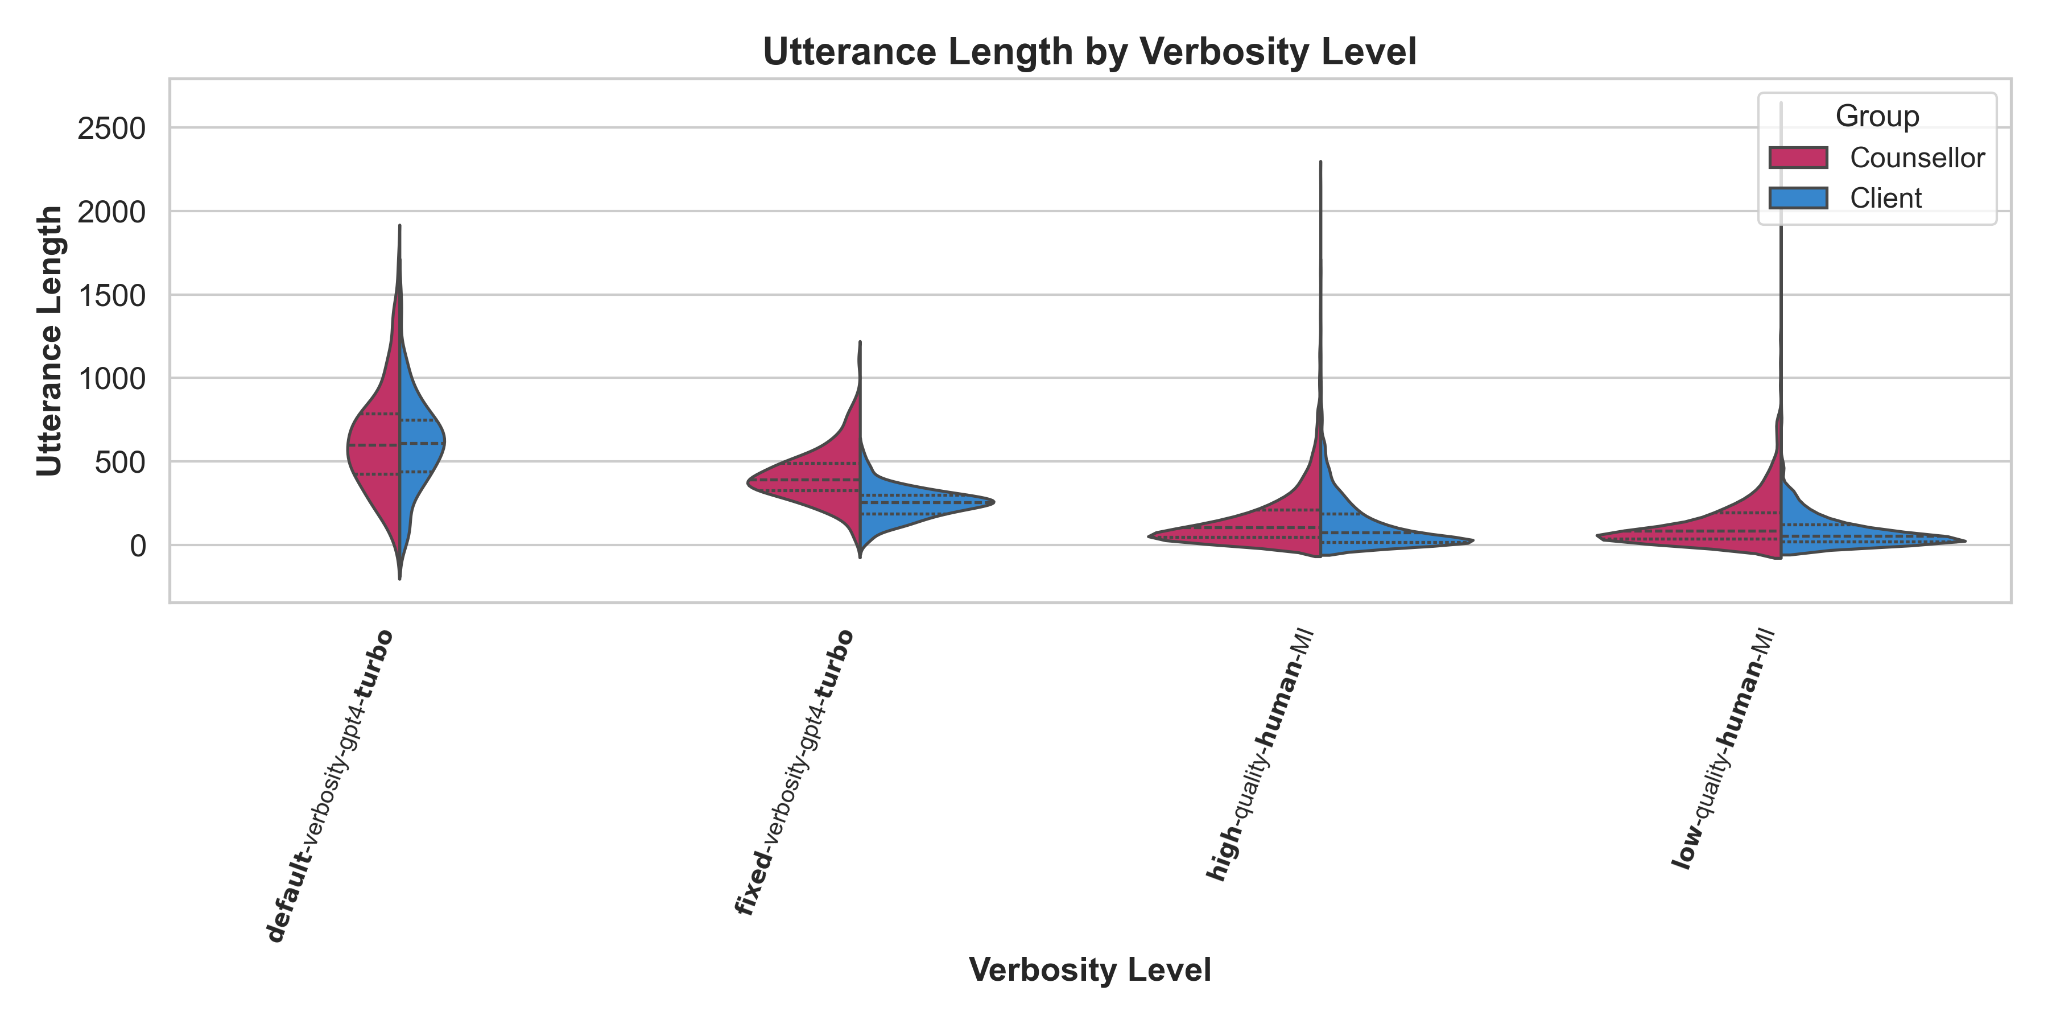
\includegraphics[width=0.9\textwidth]{figures/ch-synthetic/verbosity-comparison.png}
    \caption{Comparison of utterance length distributions between Default Verbosity, Fixed Verbosity, and Human MI conversations. The Fixed Verbosity prompt successfully reduces the synthetic smoker's (Client) utterance length to better align with human data. [PLACEHOLDER FOR FIGURE - Verbosity Slides]}
    \label{fig:verbosity-comparison}
\end{figure}

The Default Verbosity condition showed a wide distribution with a high median utterance length. The Fixed Verbosity condition successfully constrained the distribution, aligning it more closely with the human clients in the HLQC datasets.

Interestingly, we observed that the counsellor bot reciprocated the client's verbosity. When the synthetic smoker spoke less, the counsellor bot also reduced its utterance length. We also verified that these prompt modifications were robust and transferable across different LLMs (GPT-4 Turbo and GPT-4 Omni).

\subsection{Installing Resistance}
\label{sec:synthetic-smoker-resistance}

Addressing the baseline smoker's high agreeableness was crucial, as resistance to change is a central element in MI.

\subsubsection{Methodology}
We hypothesized that resistance could be installed by providing the LLM with detailed backstories emphasizing different motivations and experiences. We created two distinct personas:

\begin{itemize}
    \item \textbf{High Resistance Persona:} The backstory emphasized severe life stressors, repeated failed quit attempts, skepticism towards therapy, and a strong belief that it was not the right time to quit.
    \item \textbf{Low Resistance Persona:} The backstory described recent health concerns prompting contemplation, and an open, albeit skeptical, attitude towards change.
\end{itemize}

We generated conversations (N=10 per persona) with an MI counsellor (MIBot) and employed two distinct methods to validate the installation.

\subsubsection{Validation 1: Linguistic Evidence (Change vs. Sustain Talk)}

We analyzed the transcripts to measure the proportion of Change Talk (CT) and Sustain Talk (ST).

\textbf{Results:} The analysis confirmed a clear distinction between the two personas (Table~\ref{tab:resistance-ct-st}). The High Resistance smoker used significantly more Sustain Talk (44\% vs. 9\%) and less Change Talk (31\% vs. 61\%) than the Low Resistance smoker.

% Data from "Installing Resistance to the Synthetic Smoker" Slide 6
\begin{table}[h!]
\centering
\caption[Change and Sustain Talk for High/Low Resistance Smokers]{Proportion of Change Talk, Sustain Talk, and Neutral Talk for synthetic smokers with high and low installed resistance. The table shows that the high-resistance smoker produced more sustain talk, while the low-resistance smoker produced more change talk.}
\label{tab:resistance-ct-st}
\begin{tabular}{@{}llll@{}}
\toprule
\textbf{Persona} & \textbf{Change Talk (\%)} & \textbf{Sustain Talk (\%)} & \textbf{Neutral (\%)} \\ \midrule
High Resistance & 31 & 44 & 25 \\
Low Resistance & 61 & 9 & 30 \\ \bottomrule
\end{tabular}
\end{table}

\subsubsection{Validation 2: Behavioural Evidence (Self-Reported Readiness)}

We further validated the installation by asking the synthetic smokers to complete the Readiness Ruler survey (Importance, Confidence, and Readiness; 0-10 scale) before, immediately after, and simulated one week after the conversation.

\textbf{Methodology:} We prompted the LLM, in character, to provide numerical ratings, using Chain-of-Thought prompting (asking for reasoning before the score) to enhance reliability.

\textbf{Results:} The Readiness Ruler scores demonstrated that the synthetic smokers provided responses consistent with their installed resistance levels (Table~\ref{tab:resistance-readiness-rulers}).

% Data from "Installing Resistance to the Synthetic Smoker" Slide 11
\begin{table}[h!]
\centering
\caption[Readiness Rulers for High/Low Resistance Smokers]{Average Readiness Ruler scores (Importance, Confidence, and Readiness) for synthetic smokers with low and high installed resistance, measured at pre-conversation, post-conversation, and one-week follow-up.}
\label{tab:resistance-readiness-rulers}
\begin{tabular}{@{}l|ccc|ccc@{}}
\toprule
 & \multicolumn{3}{c|}{\textbf{Low Resistance}} & \multicolumn{3}{c}{\textbf{High Resistance}} \\
\textbf{Time Point} & \textbf{Imp.} & \textbf{Conf.} & \textbf{Ready} & \textbf{Imp.} & \textbf{Conf.} & \textbf{Ready} \\ \midrule
Pre-conversation & 4.6 & 2.6 & 3.2 & 2.0 & 1.0 & 0.6 \\
Post-conversation & 6.4 & 4.2 & 5.2 & 4.0 & 2.0 & 2.6 \\
1-Week Later & 6.6 & 4.8 & 5.4 & 4.6 & 2.6 & 3.4 \\ \midrule
Delta (Week - Pre) & 2.0 & 2.2 & 2.2 & 2.6 & 1.6 & 2.8 \\ \bottomrule
\end{tabular}
\end{table}

The High Resistance smoker reported significantly lower baseline scores. While both personas showed an increase in readiness after the MI session (Delta), the absolute levels remained distinct. This experiment demonstrated that LLMs could provide coherent self-reported behavioral data consistent with their installed attributes.

\section{Scaling Attributes and the Doppelgänger Methodology}
\label{sec:synthetic-smoker-doppelganger}

Having established control over foundational attributes, the next challenge was to scale the creation of synthetic smokers to encompass a wider range of human attributes and to develop a more rigorous validation method using real human data. This led to the development of the \textit{Doppelgänger Methodology}. It is crucial to emphasize that this methodology is not an end goal in itself, but rather a stringent strategy for \textit{validation}.

\subsection{Identifying Key Metrics: Percentage Change Talk}

To validate doppelgängers effectively, a robust, objective metric grounded in conversational language was needed. We identified the Percentage Change Talk (CF, or \%CT, calculated as CT / (CT + ST)) as a primary candidate, as it is strongly associated with behavioral change outcomes in MI.

\subsubsection{Rationale}
If CF is a valid proxy for a client's internal state, it should correlate with established metrics of readiness in human participants.

\subsubsection{Methodology and Results}
We analyzed the data from the MIBot v6.3A study (N=106 participants)~\citep{mahmood-etal-2025-fully}. The analysis confirmed strong, statistically significant correlations between CF and all readiness rulers (Table~\ref{tab:ct-correlation}). For example, the correlation with Post-conversation confidence was 0.41 ($p < 0.0001$). This established CF as a crucial, language-based metric for validation.

% Data from "Finding Smoker Attributes that Correlate with Change Talk" Slide 5
\begin{table}[h!]
\centering
\caption[Correlation of Change Fraction with Human Smoker Attributes]{Correlation between Percentage Change Talk (CF) and various human smoker attributes from the MIBot dataset (N=106). The table shows a strong positive correlation between the language used by participants and their self-reported readiness and motivation.}
\label{tab:ct-correlation}
\begin{tabular}{@{}ll@{}}
\toprule
\textbf{Attribute} & \textbf{Correlation with CF} \\ \midrule
Post-conversation Importance & 0.49 (****) \\
Post-conversation Readiness & 0.48 (****) \\
Pre-conversation Importance & 0.47 (****) \\
Post-conversation Confidence & 0.41 (****) \\
Change in Confidence (Post - Pre) & 0.24 (**) \\
CARE (Perceived Empathy) & 0.15 (ns) \\
\bottomrule
\multicolumn{2}{l}{\footnotesize{ns: P > 0.05, **: P $\le$ 0.01, ****: P $\le$ 0.0001}}
\end{tabular}
\end{table}

\subsection{The Doppelgänger Methodology}

The doppelgänger methodology leverages the MIBot dataset to validate the synthetic smoker system.

The process involves:
\begin{enumerate}
    \item \textbf{Attribute Installation:} Instantiating a synthetic smoker, $S$, by installing the known attributes of a specific human participant, $H$. Thus, $A_S = A_H$. These attributes include demographics, HSI, and pre-conversation readiness rulers.
    \item \textbf{Simulation:} The synthetic smoker $S(A_H)$ interacts with the same counsellor (MIBot) that the original human interacted with.
    \item \textbf{Comparison:} The output of the synthetic smoker, $\Gamma_S$, is compared with the actual output of the human, $\Gamma_H$.
\end{enumerate}

\subsubsection{Methodology: Attribute Installation and Validation}

We created doppelgängers for the participants (N=105) from the MIBot v6.3A study, using GPT-4 Omni. We moved from generalized backstories to direct installation of specific attributes.

\begin{verbatim}[fontsize=\small]
... About you: You are a 48-year-old male. You typically smoke 20
cigarettes per day... Before speaking to the counsellor,
you have rated your motivation... Importance: 7, Confidence: 6, Readiness: 8.
\end{verbatim}

Initial attempts using only these attributes yielded insufficient correlation in CF. To improve linguistic fidelity, we augmented the prompt with a brief, qualitative description summarizing the human's original C:S ratio (effectively adding CF to the installed attributes $A_S$).

\textbf{Results:} We calculated the Spearman correlation between human and doppelgänger outcomes (Table~\ref{tab:doppelganger-correlations}).

% Data from "Effect of Good vs. Poor-Quality Therapy" Slide 7
\begin{table}[h!]
\centering
\caption[Individual-level Validation of Doppelgänger Installation]{Individual-level validation showing the Spearman correlation of various outcome metrics between human participants and their doppelgängers (N=105) after a refined attribute installation process.}
\label{tab:doppelganger-correlations}
\begin{tabular}{@{}lll@{}}
\toprule
\textbf{Metric} & \textbf{Spearman's Coeff.} & \textbf{Significance Level} \\ \midrule
Change Fraction (CF) & 0.57 & **** \\
Change in Confidence ($\Delta$Conf) & 0.25 & * \\
CARE Score (Empathy) & 0.00 & ns \\ \bottomrule
\multicolumn{3}{l}{\footnotesize{ns: P > 0.05, *: P $\le$ 0.05, ****: P $\le$ 0.0001}}
\end{tabular}
\end{table}

The results showed a strong correlation for Change Fraction (0.57), indicating successful installation of linguistic behavior. The correlation for Change in Confidence was weaker (0.25), and there was no correlation for the CARE score.

At the population level, analysis revealed discrepancies. The mean CF for Doppelgängers (Mean=0.76) was substantially higher than that of the original human participants (Mean=0.59).

% Placeholder for Figure: CF Distribution Plots (Data from "Effect of Good vs. Poor-Quality Therapy" Slides 10/11)
\begin{figure}[ht]
    \centering
    % \includegraphics[width=0.9\textwidth]{figures/ch-synthetic/cf-distribution.png}
    \caption{Distribution of Change Fraction (CF) for Human Participants (Mean=0.59) and Synthetic Smoker Doppelgängers (Mean=0.76). [PLACEHOLDER FOR FIGURE - Good vs Bad Therapy Slides]}
    \label{fig:cf-distribution}
\end{figure}

This suggests that while the relative tendencies were captured, the synthetic smokers were generally more inclined towards change talk than their human counterparts.

\section{Evaluating the Utility of Synthetic Smokers}
\label{sec:synthetic-smoker-utility}

Having developed a method to create synthetic smokers with validated linguistic fidelity, the final step was to confirm their utility. To be useful for testing systems and training humans, synthetic smokers must be sensitive to the quality of the counselling they receive.

\subsection{Sensitivity to Counselling Quality}

\textbf{Rationale:} We designed an experiment to test if validated doppelgängers exhibit differential responses to high-quality MI versus low-quality, confrontational counselling.

\subsubsection{Methodology}

\textbf{1. Sampling:} We created two participant groups (N=25 each) based on their actual Change Fraction (CF) in the MIBot study: High-CF (top 25th percentile) and Low-CF (bottom 25th percentile).

\textbf{2. Doppelgänger Creation:} We created doppelgängers for these 50 participants using the validated methodology.

\textbf{3. Counsellor Conditions:} We exposed these doppelgängers to two different automated counsellors:
\begin{itemize}
    \item \textbf{Good MI Counsellor (MIBot v6.3A):} A high-quality, MI-adherent chatbot.
    \item \textbf{Bad (Confrontational) Counsellor:} An LLM prompted to be directive, judgmental, and confrontational (e.g., ``Giving advice without being asked,'' ``Trying to persuade them to quit...'').
\end{itemize}

\textbf{4. Measurement:} We measured CF, $\Delta$Confidence (simulated week later), and the CARE score reported by the doppelgänger.

\subsubsection{Results}

The results (Table~\ref{tab:good-vs-bad-counselling}) demonstrated that the synthetic smokers were highly sensitive to the quality of counselling.

% Data from "Effect of Good vs. Poor-Quality Therapy" Slide 19
\begin{table}[h!]
\centering
\caption[Doppelgänger Outcomes with Good vs. Bad Counselling]{Outcomes for doppelgängers when interacting with a good (MIBot 6.3A) versus a bad (confrontational) automated counsellor. The table shows that doppelgängers exhibited different behaviors and outcomes based on the quality of the counselling they received.}
\label{tab:good-vs-bad-counselling}
\begin{tabular}{@{}llccc@{}}
\toprule
\textbf{Counsellor} & \textbf{Participant Group} & \textbf{CF} & \textbf{$\Delta$Confidence} & \textbf{CARE} \\ \midrule
\multirow{2}{*}{Good (MIBot 6.3A)} & High-CF Doppelgängers & 0.80 & 1.4 & 49.8 \\
 & Low-CF Doppelgängers & 0.48 & 1.1 & 47.8 \\ \midrule
\multirow{2}{*}{Bad (Confrontational)} & High-CF Doppelgängers & 0.68 & 1.1 & 41.0 \\
 & Low-CF Doppelgängers & 0.22 & 0.5 & 23.0 \\ \bottomrule
\end{tabular}
\end{table}

When interacting with the Bad counsellor, outcomes were significantly worse across all metrics. CF dropped markedly, particularly for the Low-CF group (from 0.48 to 0.22), indicating increased resistance. The Change in Confidence was lower, and the CARE scores showed the most dramatic difference (e.g., 23.0 vs. 47.8 for the Low-CF group).

These results confirm that the synthetic smokers behave realistically, reacting negatively to poor-quality counselling. This sensitivity validates their utility as evaluation and training tools.

\section{Discussion and Limitations}

This chapter detailed the iterative development and validation of Synthetic Smokers, demonstrating significant progress in simulating human behaviour for clinical applications. The research highlights the evolution of validation methodologies, moving from human inspection to the rigorous Doppelgänger framework.

\subsection{Comparison with Prior Work}

The concept of simulated patients has existed for decades (see Sections 2.4-2.6). Early approaches often relied on rule-based systems or scripted responses, which lacked the flexibility and realism required for complex interactions like MI. More recent approaches utilizing LLMs have shown promise in generating realistic dialogue~\citep{cheng2023gpatients}, but often lack the rigorous, attribute-specific validation against human behavioral data presented here. Our approach advances the field by focusing on creating validated digital behavioral twins using established clinical metrics (\%CT, Rulers) and demonstrating their sensitivity to intervention quality.

\subsection{Limitations}

Despite the progress, several limitations remain.

\subsubsection{The Caricature Effect and Incongruous Personas}

LLMs often rely on stereotypical representations, leading to a "caricature effect." This bias might be exacerbated when attempting to simulate "incongruous" personas—individuals whose views do not align with the stereotypes of their demographic (e.g., a political liberal who supports increased military spending). Recent research suggests LLMs are less steerable towards incongruous personas~\citep{liu2024evaluating}, indicating that current models may struggle to capture the full nuance of human beliefs, potentially resulting in oversimplified simulations.

\subsubsection{Fidelity of Self-Reports}

While linguistic fidelity (\%CT) was high, the fidelity of self-reported internal state changes ($\Delta$Confidence) and perceptions (CARE) was lower. This suggests that while LLMs can mimic the language of change, simulating the nuanced internal psychological shifts remains a challenge.

\subsubsection{Population-Level Biases}

The Doppelgängers exhibited a higher overall \%CT than the human population they were modeled on, suggesting a potential bias towards agreeableness or optimism in the LLM that was not fully mitigated by the installation process.

\section{Conclusion}

This chapter detailed the development of synthetic smokers, establishing a clear vision and a formal framework ($A_S \rightarrow \Gamma_S$) for their creation and validation. Through an iterative process, we demonstrated the successful installation of foundational attributes and developed the Doppelgänger methodology for rigorous validation. We showed that crucial linguistic markers (\%CT) can be reliably installed and that these agents are sensitive to the quality of counseling. The development of validated synthetic smokers provides a powerful and scalable tool for testing automated systems and training human clinicians, advancing the field of digital health interventions.